\pagenumbering{arabic}

\chapter{Introduction} \label{introduction}


\section{Purpose of the System }
The FarmBot system is designed to automate and optimize small-scale agricultural tasks, embodying the principles of precision farming and sustainability. Through its open-source CNC farming machine, FarmBot aims to:
\begin{itemize}
    \item Automate planting, watering, weeding, and monitoring of plant health to reduce labor and increase efficiency.
    \item Employ precision farming techniques to optimize resource use and enhance crop yields, promoting sustainability.
    \item Offer customizability and flexibility, enabling users to tailor the system to their specific agricultural needs.
    \item Serve as an educational tool, facilitating hands-on learning in STEM fields and sustainable agricultural practices.
    \item Foster a community-driven approach to innovation in agriculture, encouraging collaboration and continuous improvement.
\end{itemize}
This system’s purpose aligns with advancing sustainable, efficient, and accessible agriculture through technological innovation.

\section{Scope}

The scope of the FarmBot software encompasses several key modules designed to automate and optimize agricultural operations on a small scale. These modules include:

\begin{itemize}
    \item \textbf{Plant Scheduler}: Automates the planting process by scheduling tasks based on crop types and planting patterns.
    \item \textbf{Water Management System}: Optimizes water usage by adjusting watering schedules in response to soil moisture levels and weather forecasts.
    \item \textbf{Weed Detection and Control}: Employs image recognition to identify and manage weed growth with minimal human intervention.
    \item \textbf{Health Monitoring}: Utilizes sensor data to monitor plant health and soil conditions, providing actionable insights to users.
    \item \textbf{User Interface (UI)}: Offers a web-based interface for users to interact with FarmBot, customizing settings, monitoring operations, and receiving updates.
\end{itemize}

These software products facilitate the core functionalities of FarmBot, enabling efficient, automated farming operations. They are designed to:

\begin{itemize}
    \item Reduce manual labor and operational complexity in gardening and small-scale farming.
    \item Enhance crop yields and sustainability by optimizing resource usage and environmental adaptation.
    \item Provide educational opportunities through hands-on engagement with agricultural technology.
\end{itemize}

The application of FarmBot's software is targeted at individual gardeners, educators, and small-scale farmers, offering significant benefits such as increased efficiency, sustainability, and accessibility to precision agriculture. The objectives and goals of this project align with promoting sustainable farming practices, advancing agricultural education, and fostering a community of innovation in farming technology. This scope is consistent with the higher-level specifications outlined in the system requirements, focusing on the integration of technology into agriculture to meet modern demands for food production and environmental stewardship.

\section{System Overview}
\subsection{System Perspective}
FarmBot is a standalone, autonomous precision agriculture system that enhances small-scale gardening through automation. FarmBot epitomizes the forefront of autonomous precision agriculture technology, designed to transform small-scale gardening through automation. It leverages external data sources, such as weather forecasts and agricultural databases, to offer an all-encompassing garden management interface. The system combines precision-engineered hardware components with an intuitive web-based software platform and supports both Wi-Fi and Ethernet for robust internet connectivity. Capable of performing a wide range of operations from seeding to plant health monitoring, FarmBot's design is inherently adaptable, facilitated by a modular construction that allows for the integration of additional sensors and tools, enhancing its capabilities over time.

\begin{figure}[H]
    \centering
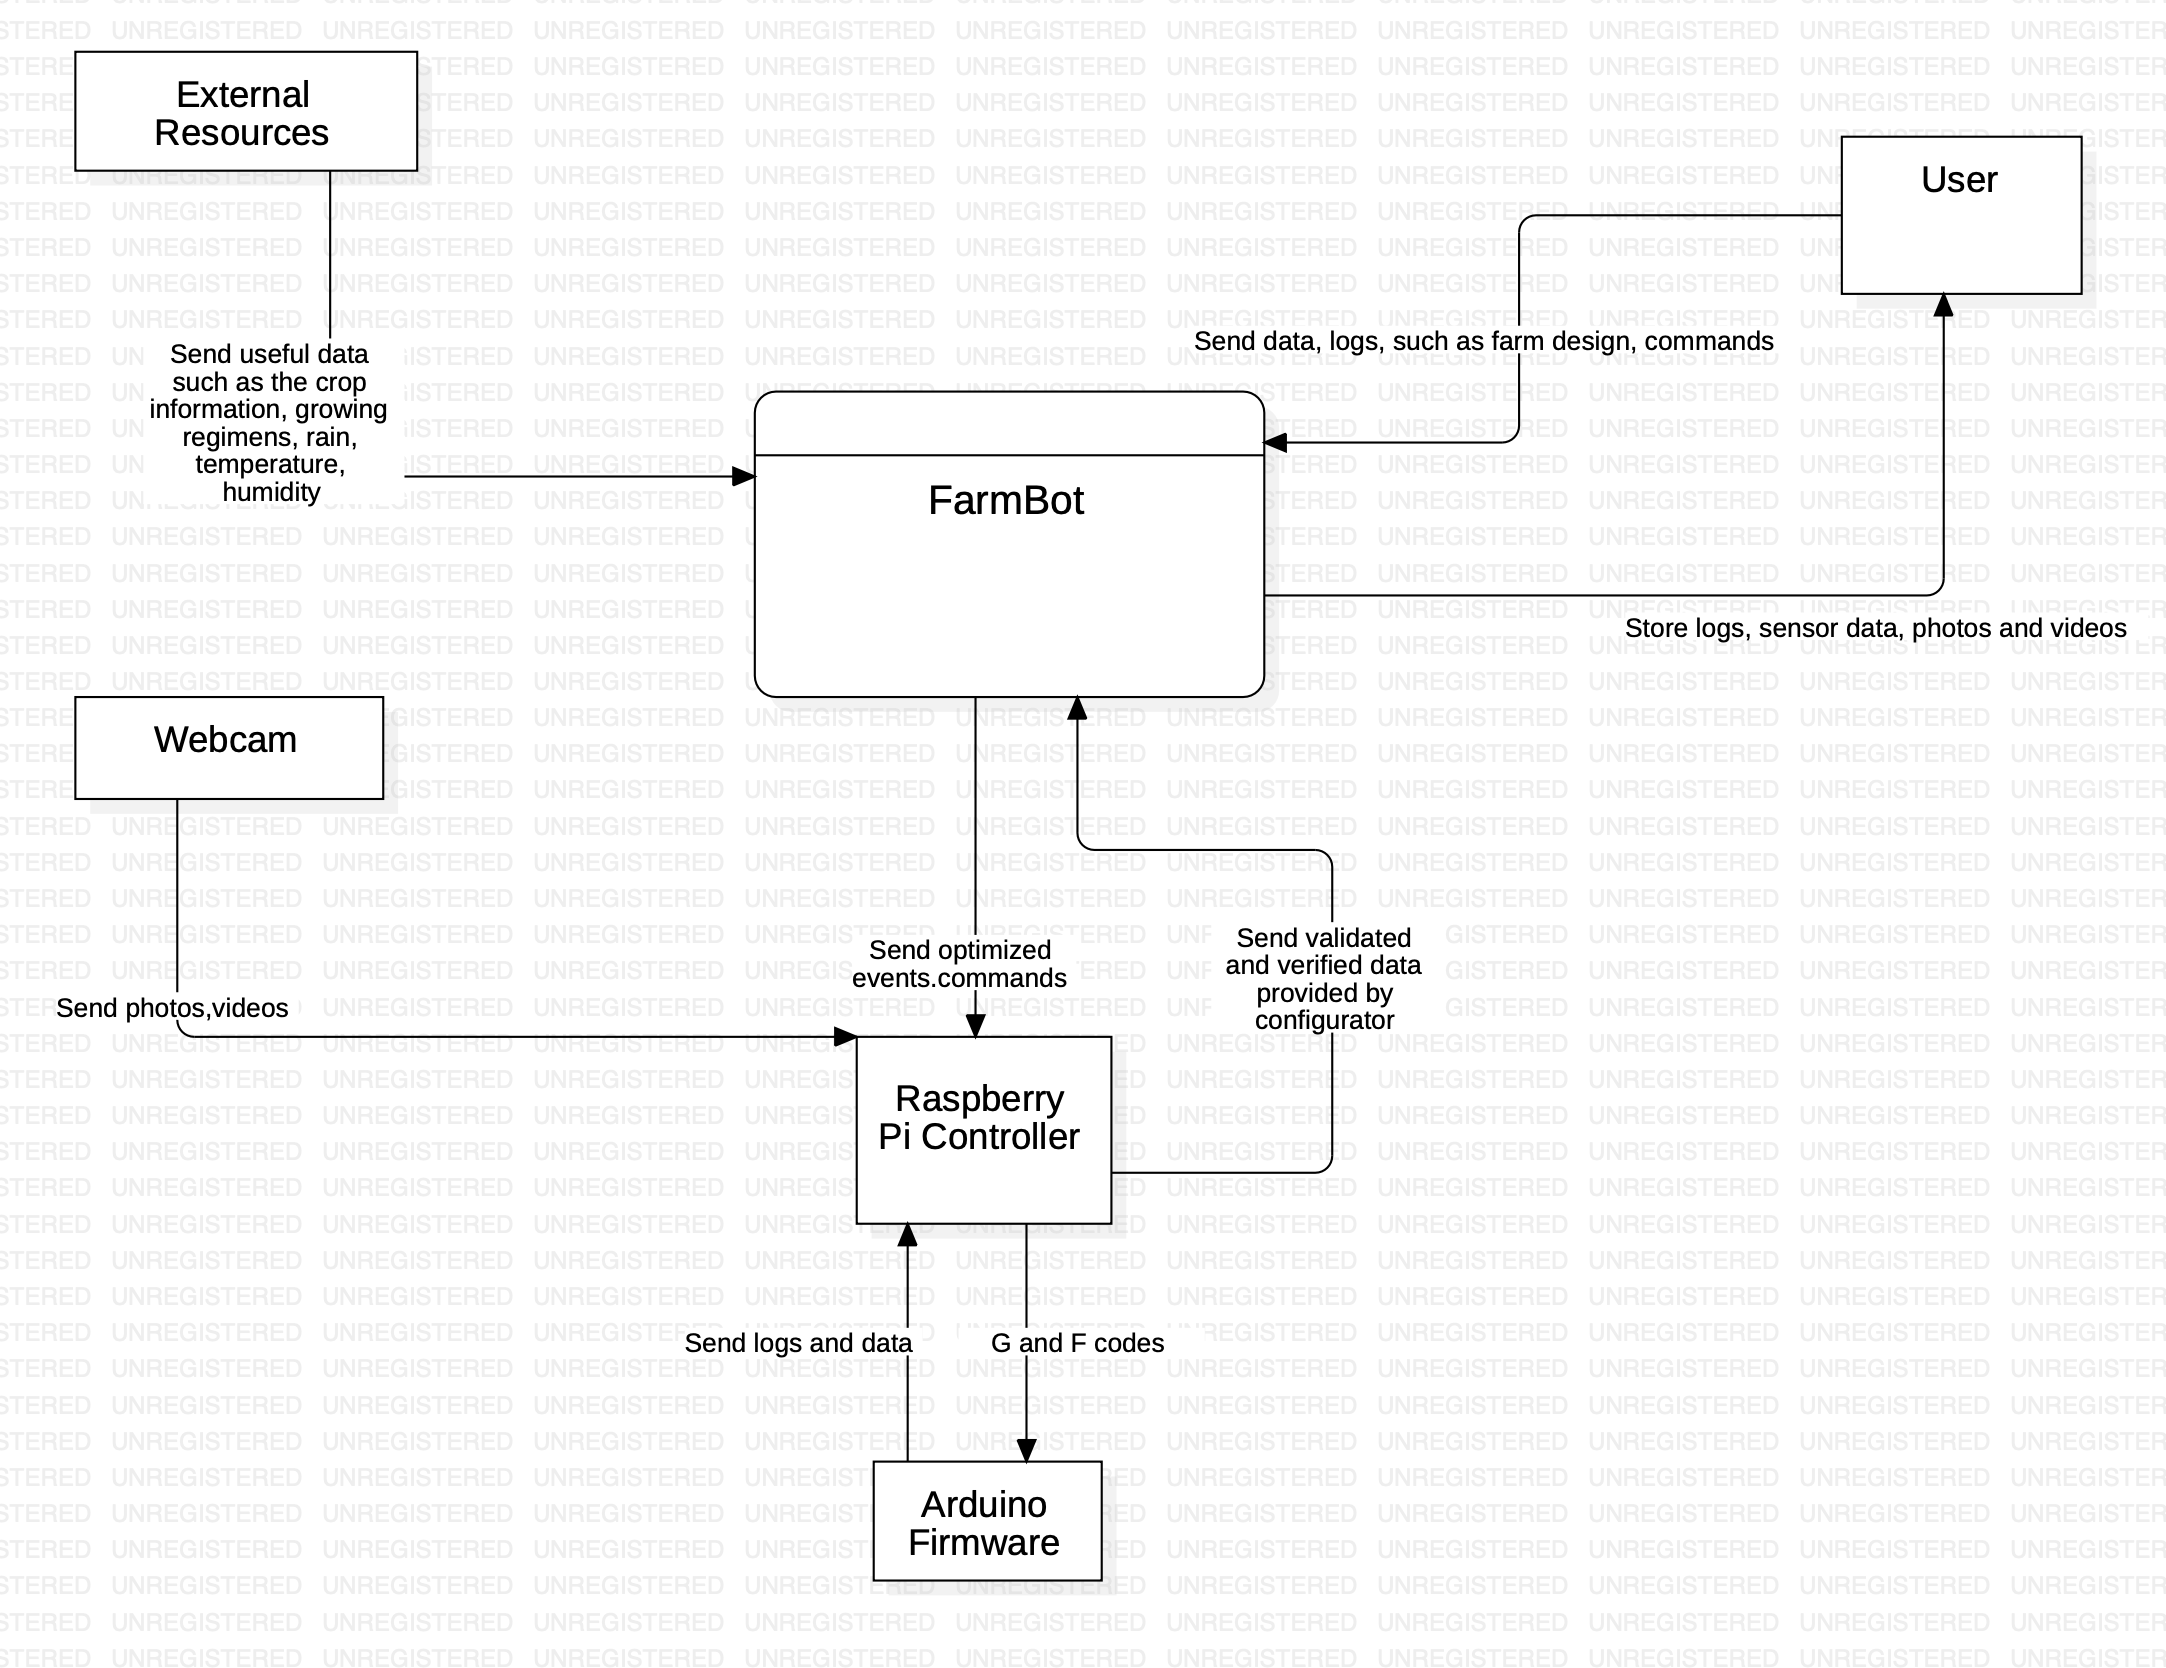
\includegraphics[scale=0.2]{./Figures/farmbot_context_diagram.png}
\caption{FarmBot Context Diagram}
\end{figure}

\subsubsection{System Interfaces}
FarmBot's system interfaces facilitate the seamless operation of hardware components and external data exchange, encompassing connections between the microcontroller and various sensors and actuators. These interfaces are governed by industry standards such as SPI and I2C for sensor data communication, ensuring reliable and efficient data transfer. Additionally, interfaces with external databases and cloud storage adhere to secure web standards, including HTTPS and RESTful APIs, to protect data integrity and privacy.

\begin{figure}[H]
    \centering
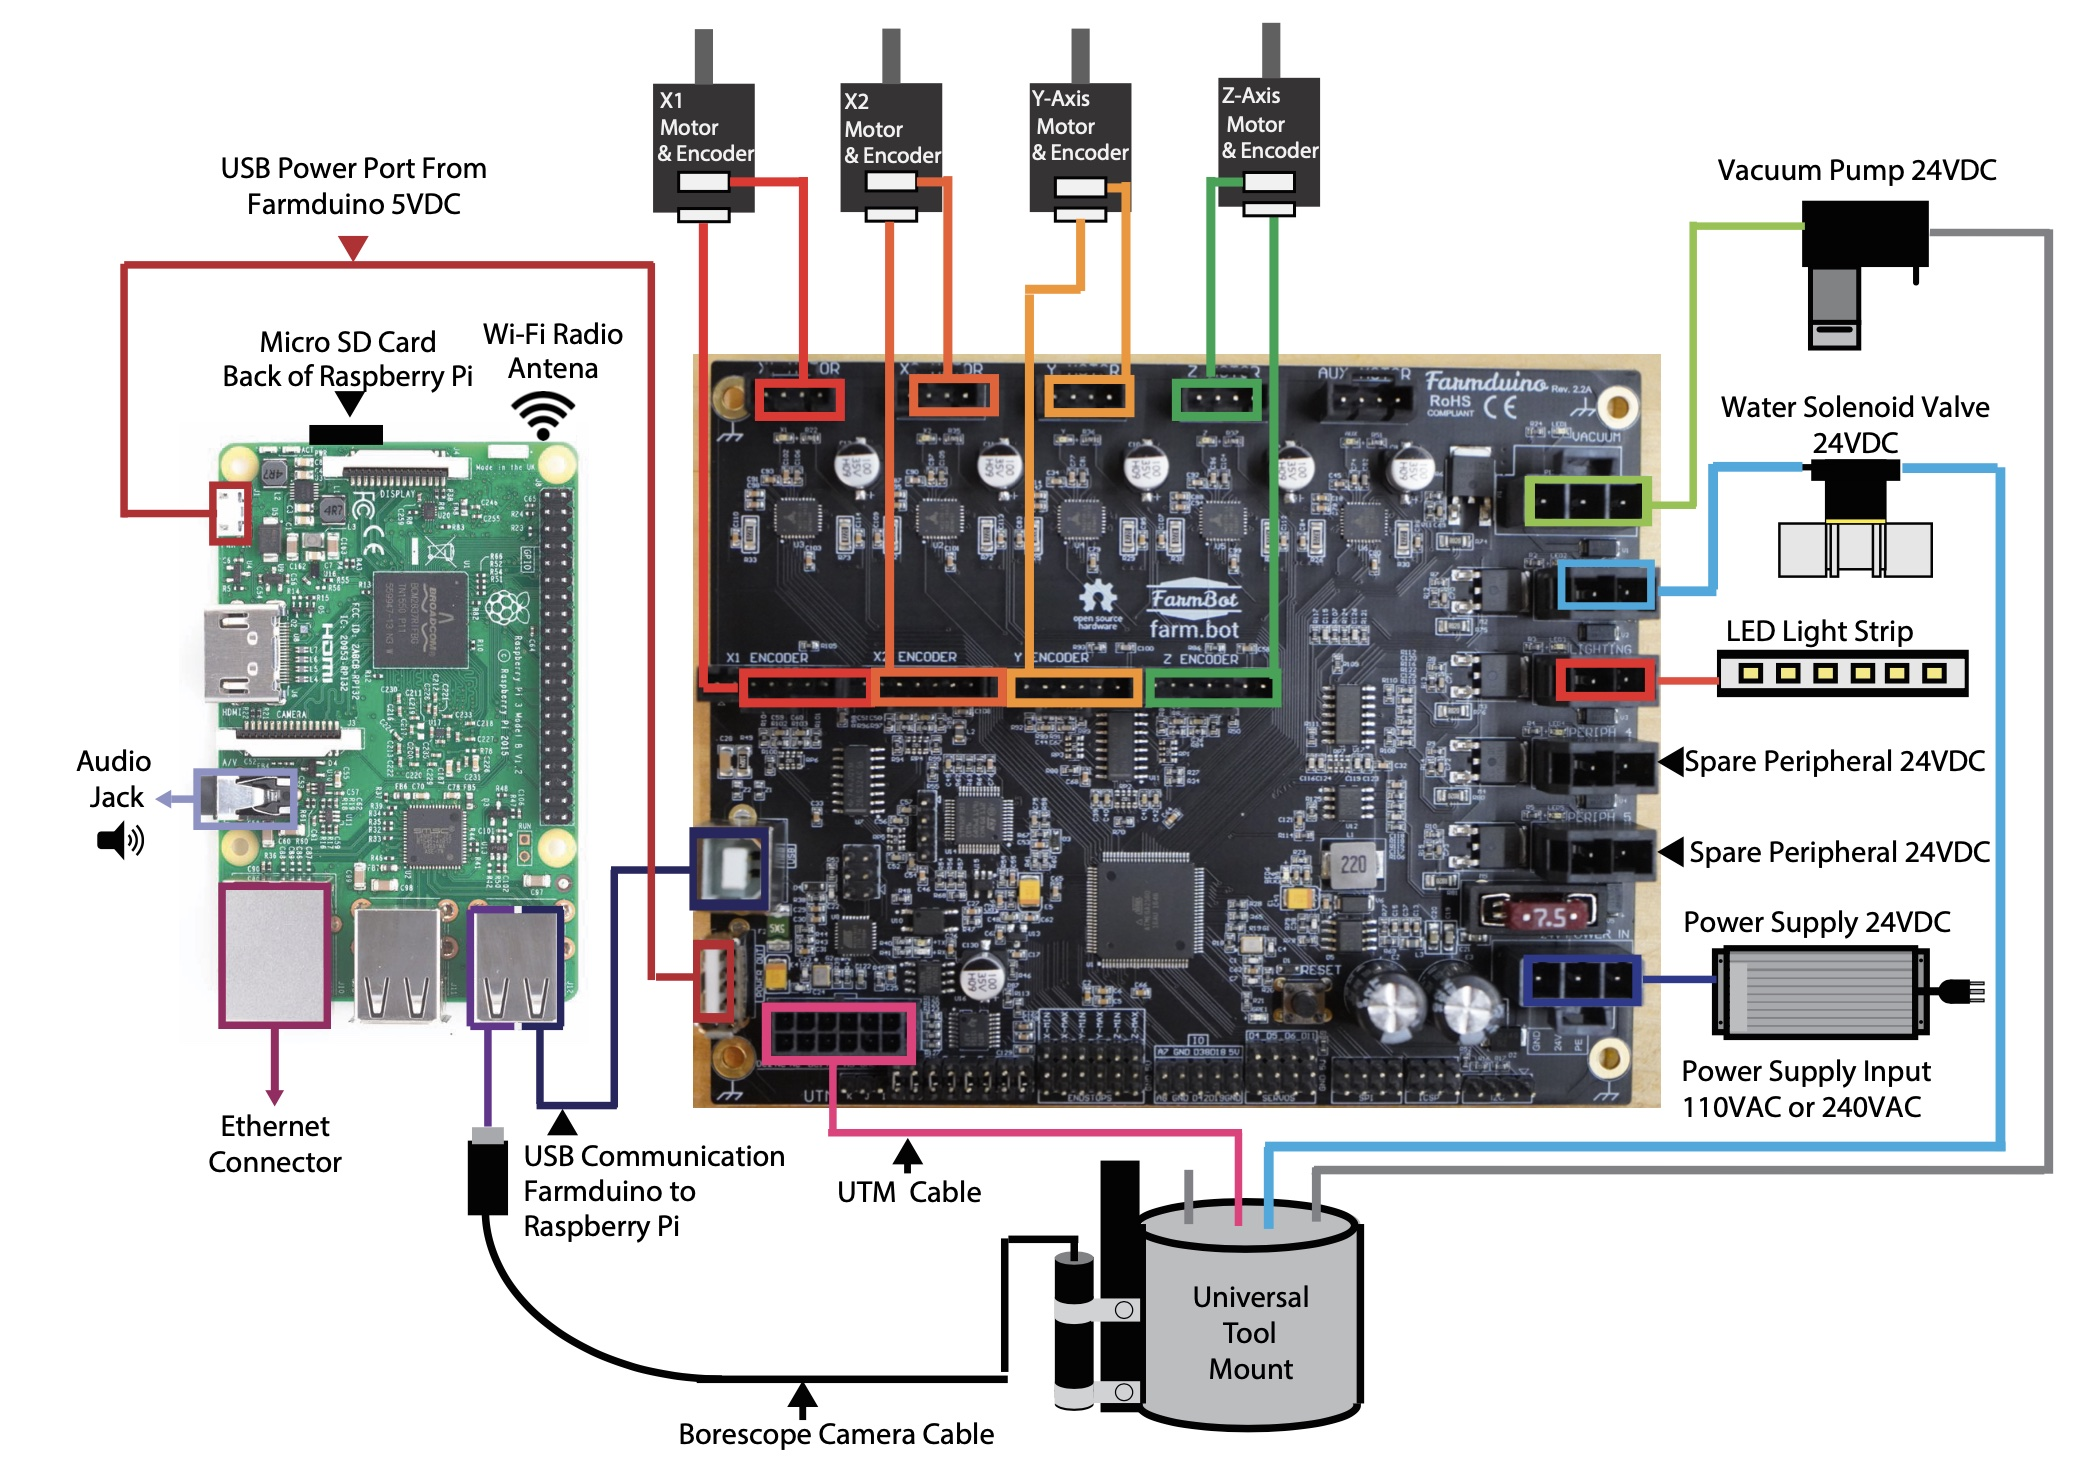
\includegraphics[scale=0.2]{./Figures/farmbot_system_diagram.jpeg}
\caption{FarmBot System Diagram}
\end{figure}

\subsubsection{User Interfaces}
The user interfaces of FarmBot, including a web application and mobile app, are designed for ease of use and accessibility, enabling users to remotely control, monitor, and configure their FarmBot systems. These interfaces comply with web accessibility standards (WCAG) and best practices in UI/UX design, ensuring a seamless and inclusive user experience across different devices and platforms.

\begin{figure}[H]
    \centering
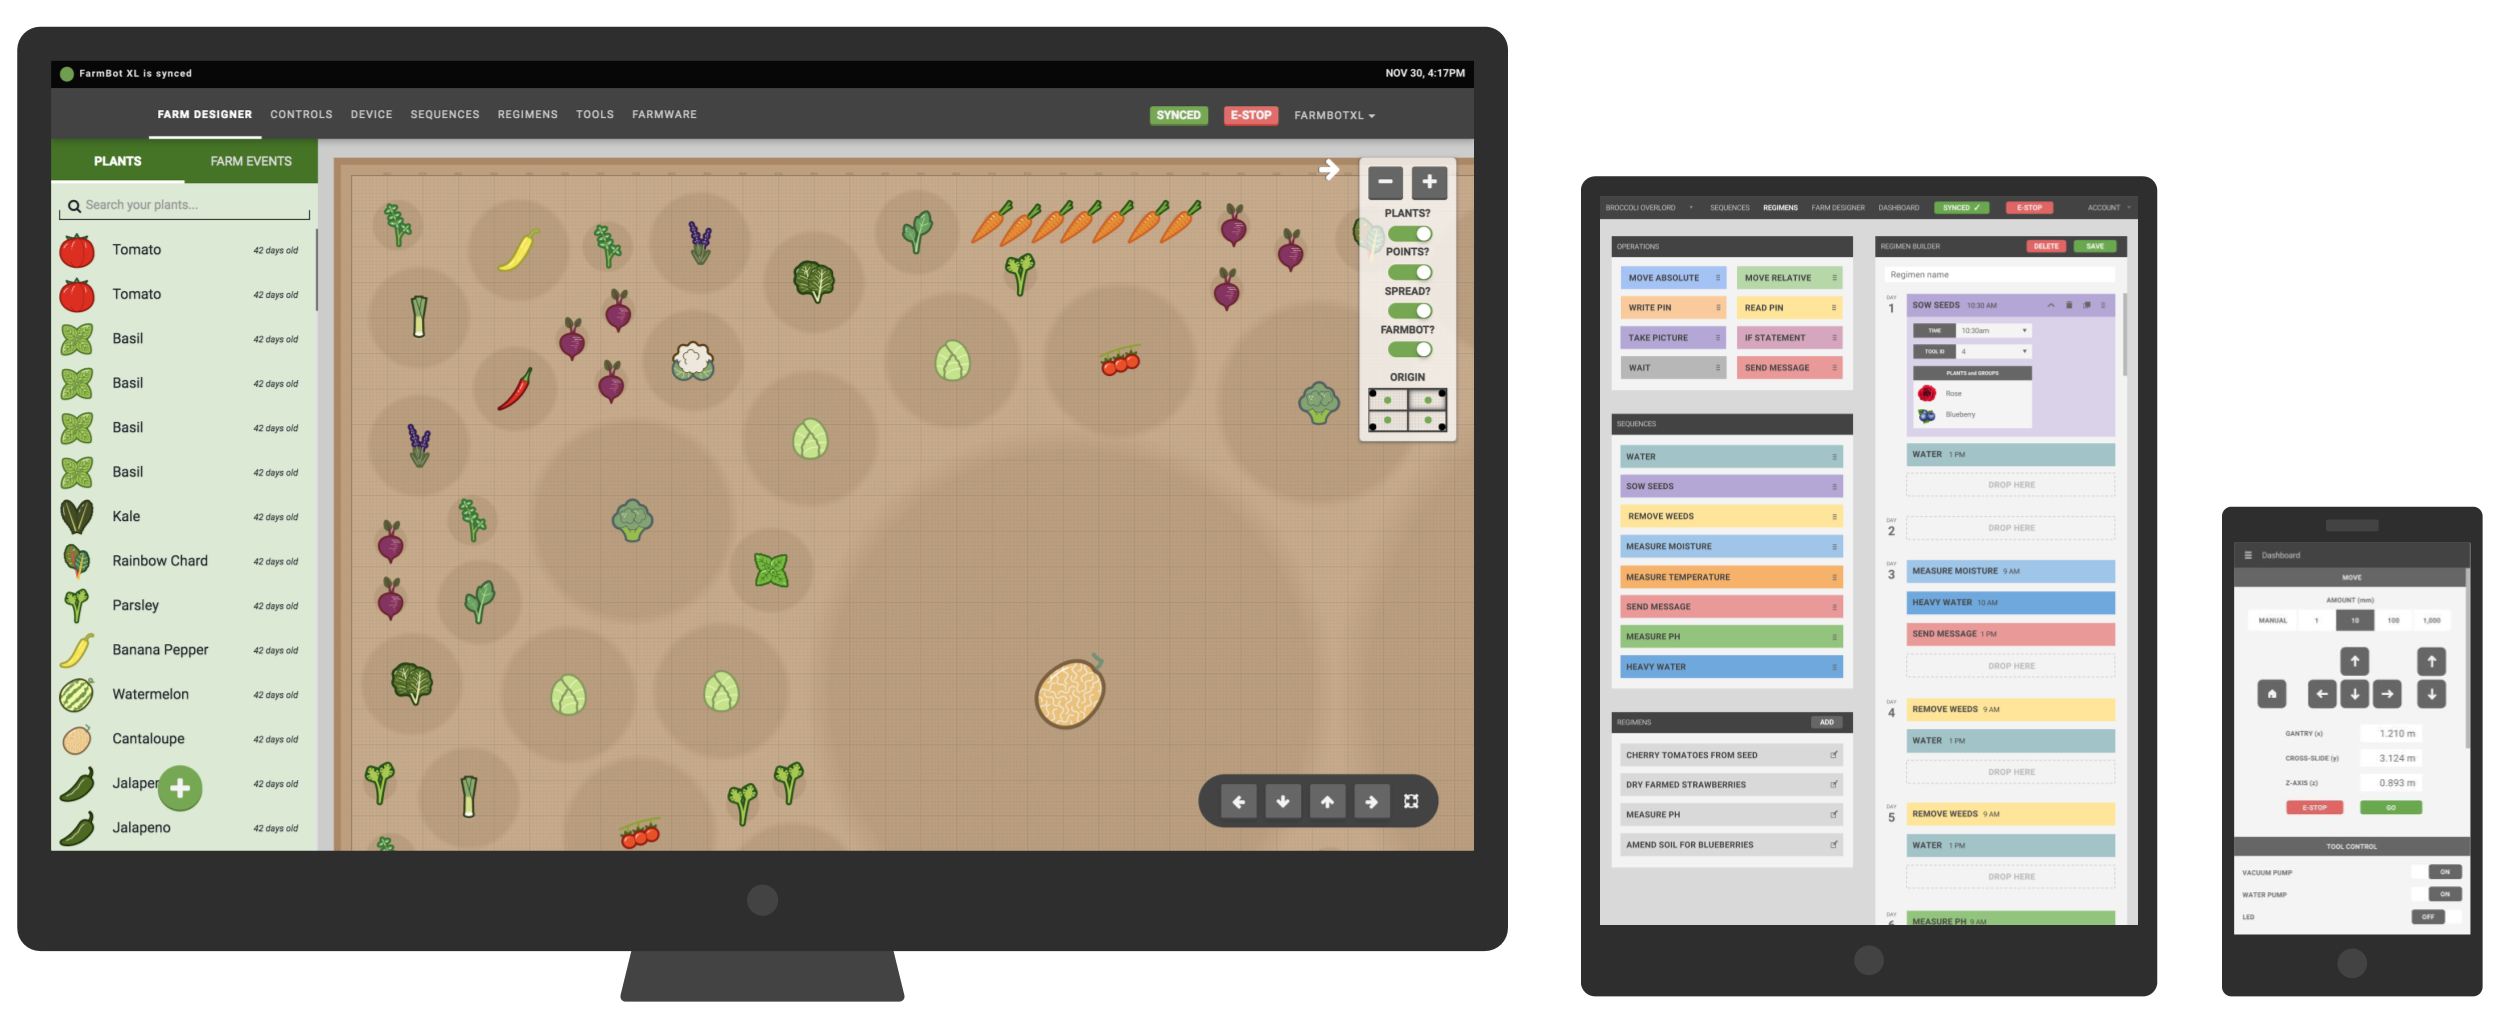
\includegraphics[scale=0.2]{./Figures/farmbot_ui.png}
\caption{FarmBot Web App on Different Devices}
\end{figure}

\subsubsection{Hardware Interfaces}
FarmBot's hardware interfaces, which include connections to soil moisture sensors, the watering system, seed dispensers, and camera systems, adhere to electrical and communication standards to ensure safety and functionality.Their special Farmduino electronics board features a dedicated processor for monitoring the rotary encoders at high speed, while the Raspberry Pi 3 serves as the web-connected brain. The standards FarmBot uses here include IEEE 802 for wireless communication and USB standards for peripheral devices, ensuring compatibility and safe operation across the system's hardware components.

\begin{figure}[H]
    \centering
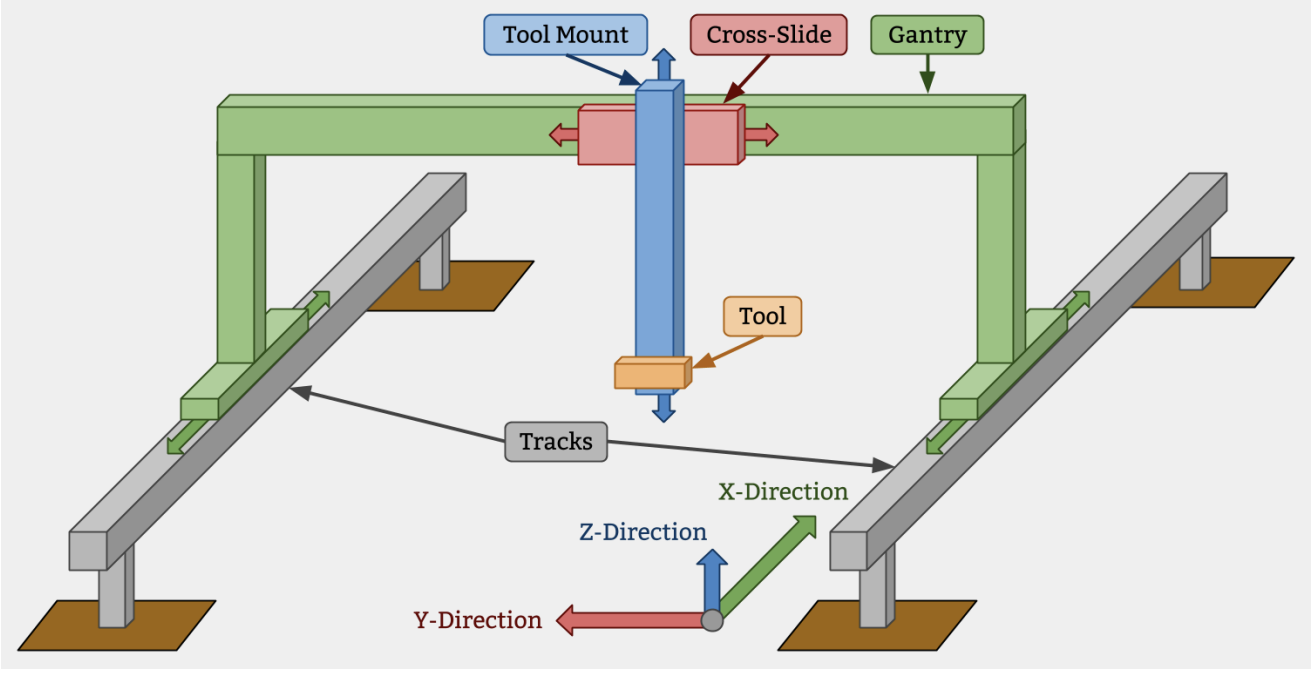
\includegraphics[scale=0.3]{./Figures/farmbot_high_level_hardware.png}
\caption{FarmBot High Level Hardware Overview and Coordinate System.}
\end{figure}

\begin{figure}[H]
    \centering
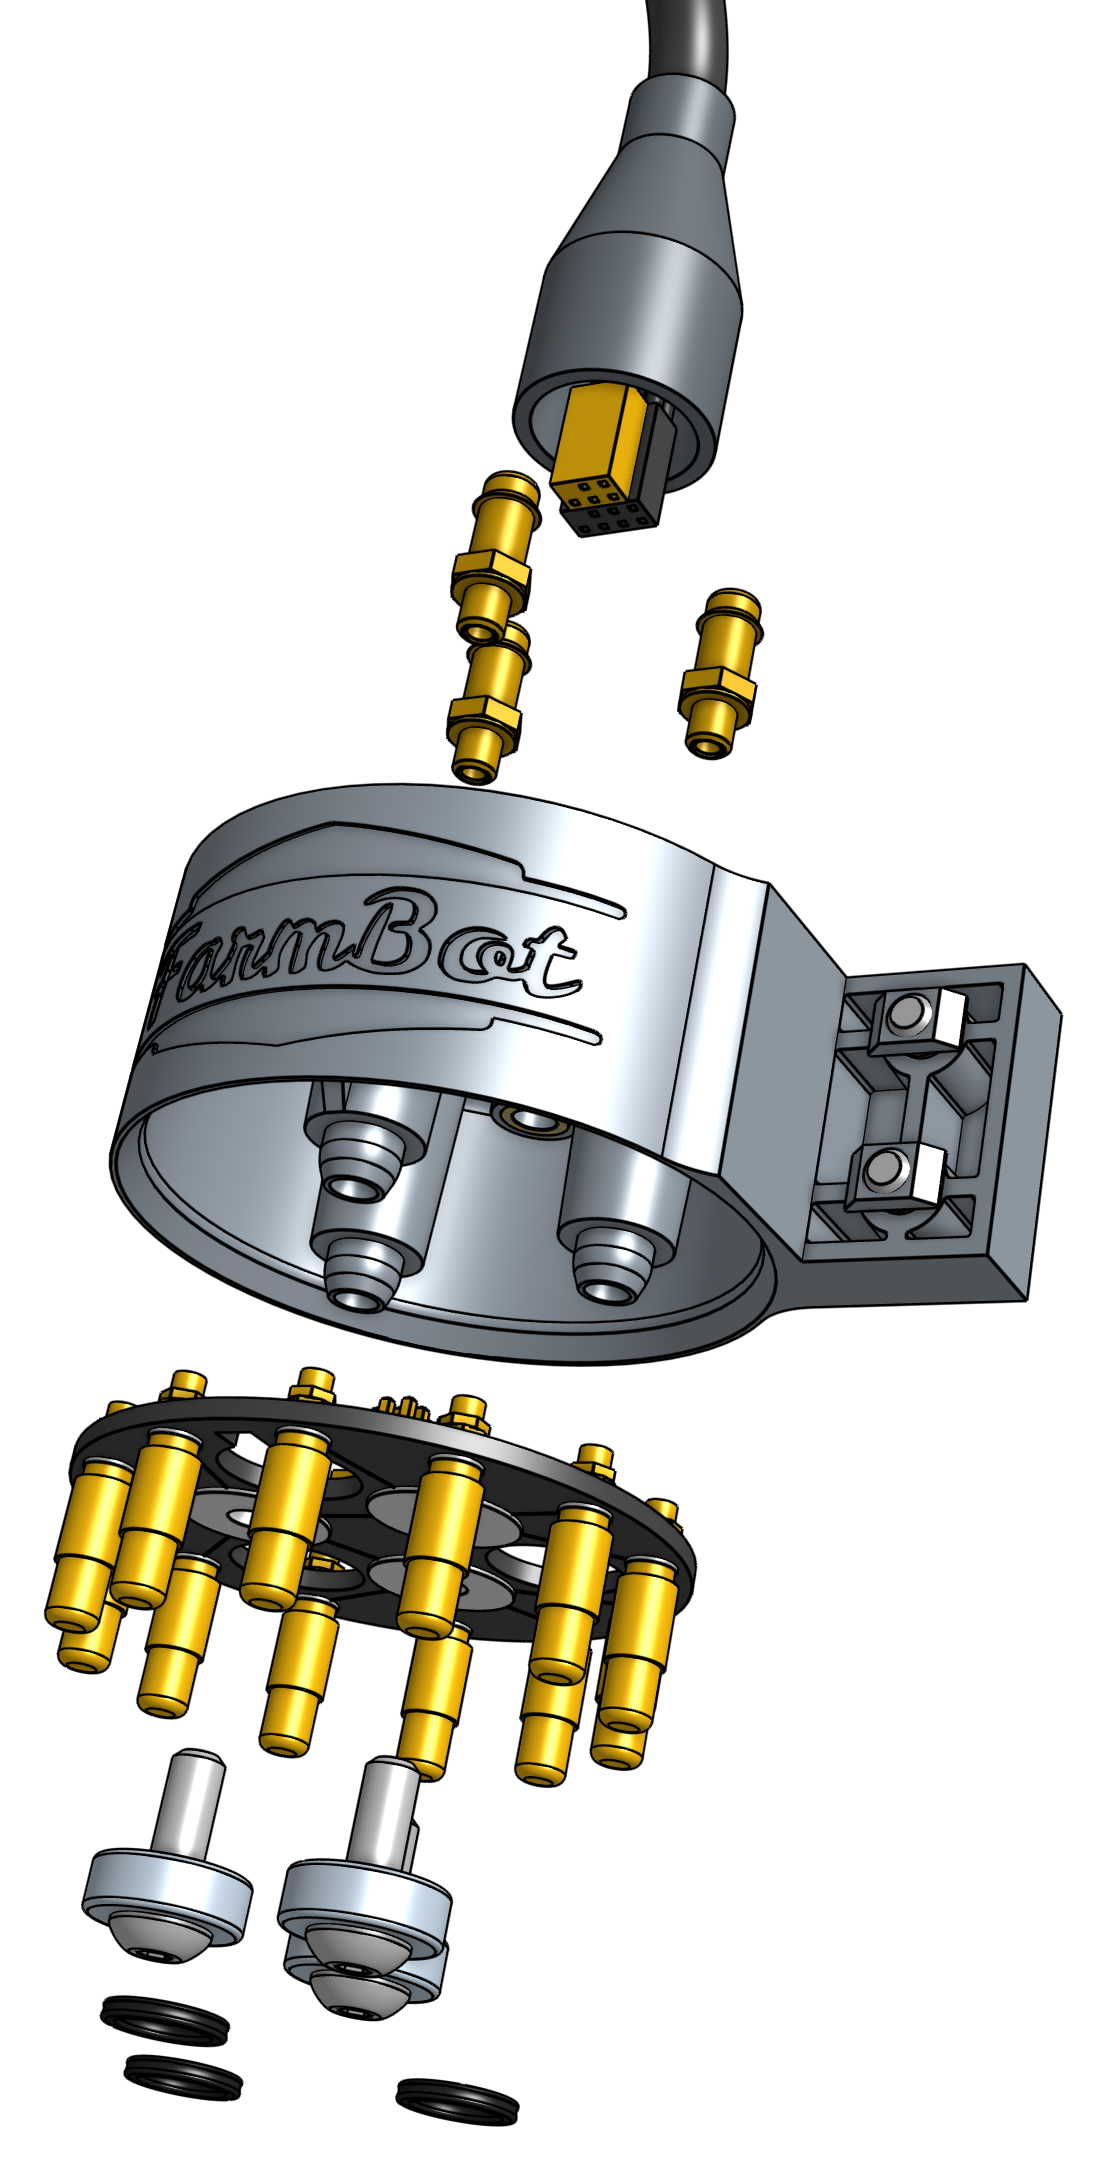
\includegraphics[scale=0.1]{./Figures/farmbot_hardware.png}
\caption{FarmBot Genesis Universal Tool Mount}
\end{figure}

\subsubsection{Software Interfaces}
The software infrastructure of FarmBot, based on a lightweight Linux operating system, supports various software interfaces for system operation and management. Compliance with open-source licensing and security standards, including the Secure Software Development Framework (SSDF) by NIST, ensures that FarmBot's software remains secure, reliable, and maintainable.FarmBot’s Raspberry Pi runs a custom operating system named FarmBot OS to maintain a connection and synchronize with the web application via the message broker. This allows FarmBot to download and execute scheduled events, be controlled in real-time, and upload logs and sensor data. The OS communicates with the Farmduino/Arduino over a USB cable or serial connection to send G and F code commands, and also receive collected data from sensors and rotary encoders.FarmBot OS has a built-in utility named configurator allowing you to easily enter WiFi and web app credentials from a WiFi enabled device (such as a laptop or smartphone). This is used for initial setup in order to get your FarmBot connected to your home WiFi and web app account.
The firmware that is flashed onto the Arduino or Farmduino microcontroller is responsible for physically operating FarmBot’s motors, tools, sensors, and other electronics. It receives G and F codes from FarmBot OS, and then moves the motors and reads and writes pins accordingly. It also sends collected data from the rotary encoders and pin reads back to the Raspberry Pi.\cite{farmbot2024intro}

\begin{figure}[H]
    \centering
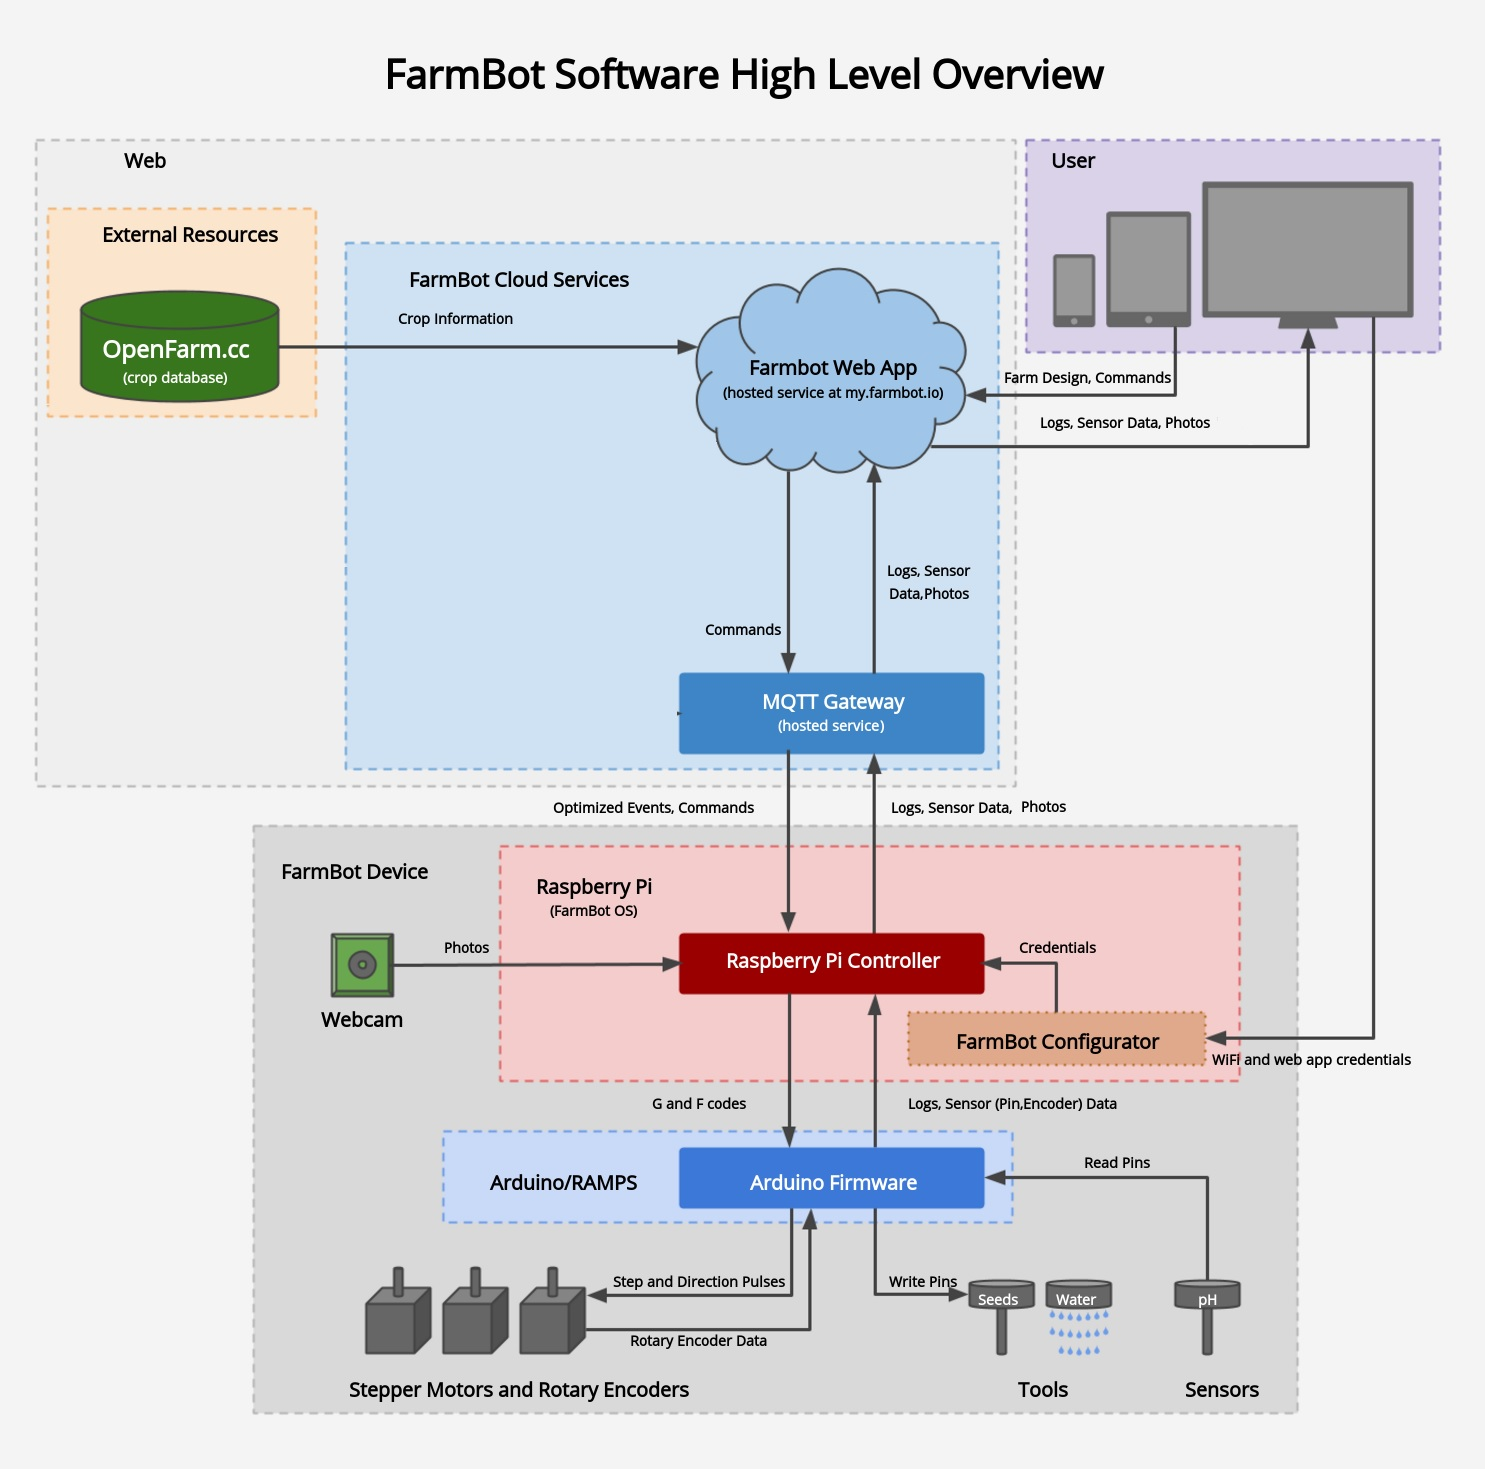
\includegraphics[scale=0.3]{./Figures/farmbot_software_high_level_overview.jpg}
\caption{FarmBot Software High Level Overview}
\end{figure}


\subsubsection{Communication Interfaces}
Communication is the lifeblood of FarmBot, enabling not just the operation of the device itself but also its interaction with the broader digital world. FarmBot uses a configurator which  is a piece of software built into FarmBot OS that makes it easy to connect your FarmBot to a WiFi network and user's web app account. FarmBot's communication interfaces, enabling Wi-Fi, Ethernet, and optional Bluetooth connectivity, are designed in accordance with IEEE standards, including IEEE 802.11 for Wi-Fi and IEEE 802.15.1 for Bluetooth. These standards ensure robust and secure data communication, allowing FarmBot to receive updates, synchronize data, and provide remote access functionalities efficiently.

\begin{figure}[H]
    \centering
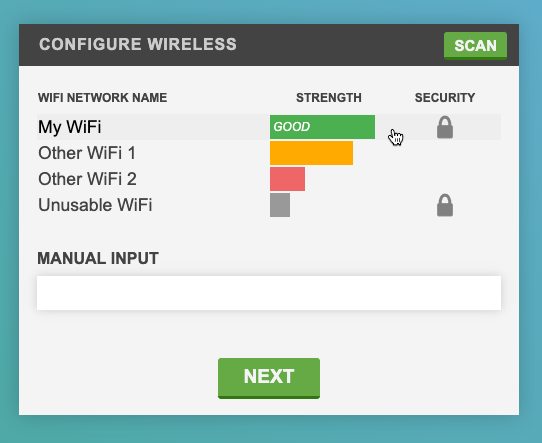
\includegraphics[scale=0.5]{./Figures/farmbot_wifi_connections.png}
\caption{FarmBot Configurator in use for Wi-Fi Connection}
\end{figure}

\subsubsection{Memory Constraints}
Addressing memory constraints, FarmBot incorporates on-board and expandable memory solutions, following industry standards for flash memory and external storage, such as SD memory card standards.An external memory interface, such as an SD card slot, offers users the flexibility to expand storage capacity. This is particularly useful for logging detailed operational data and storing images captured for plant health monitoring, ensuring that memory limitations never compromise the system's performance or data retention capabilities.

\begin{figure}[H]
    \centering
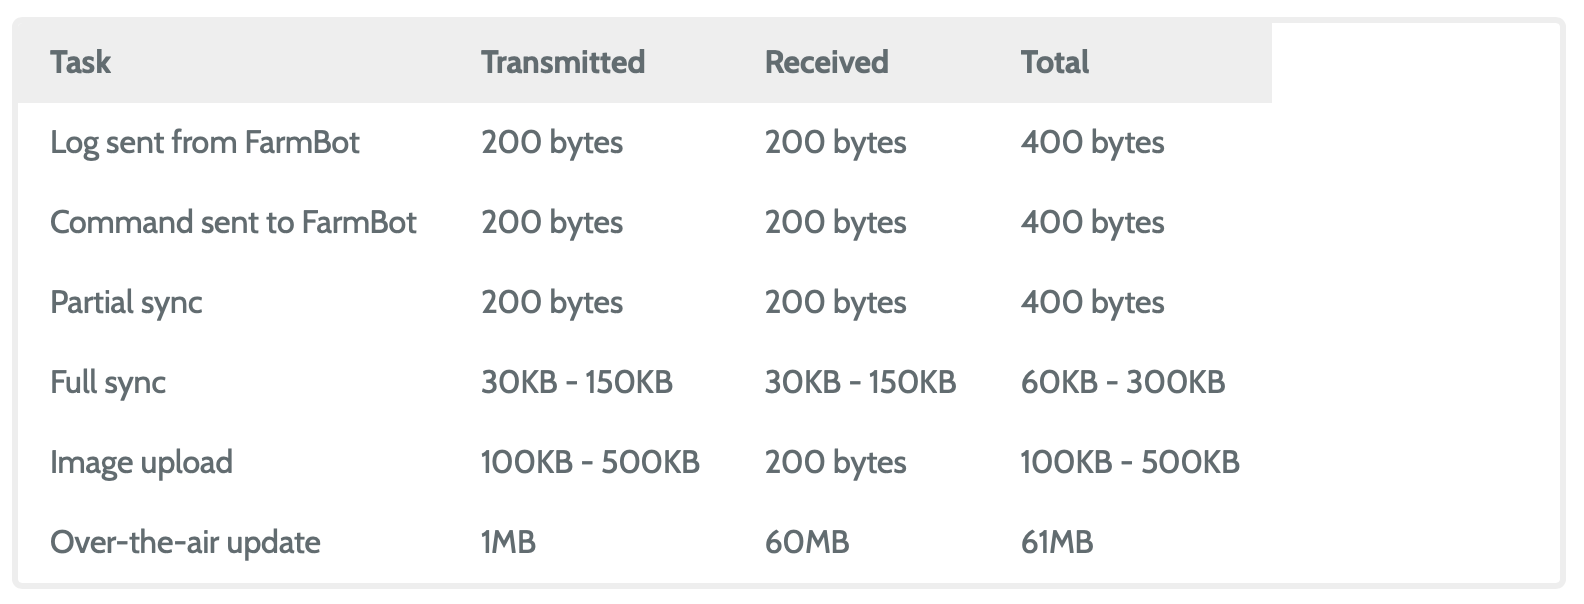
\includegraphics[scale=0.3]{./Figures/farmbot_data_required.png}
\caption{Average data required by task}
\end{figure}

\subsubsection{Operations}

This section outlines the normal and special operations required by users of FarmBot, including modes of operation, interactive and unattended periods, data processing support functions, and backup and recovery operations.

\paragraph{Modes of Operations in the User Organization}

\paragraph{User-Initiated Operations:}
\begin{itemize}
    \item \textbf{Garden Planning and Setup:} Users design their garden layout, specifying plant locations, types, and schedules using the web or mobile application.
    \item \textbf{Manual Control Mode:} Allows for direct control over FarmBot components for immediate tasks or testing purposes.
    \item \textbf{Scheduled Operations Mode:} Users schedule routine tasks such as watering, weeding, and fertilizing tailored to the garden’s needs.
\end{itemize}

\paragraph{Special Modes:}
\begin{itemize}
    \item \textbf{Monitoring and Alerts Mode:} FarmBot monitors soil moisture, plant health, and growth, alerting users to any anomalies detected.
    \item \textbf{Learning Mode:} FarmBot suggests optimizations based on historical data and machine learning algorithms (if applicable).
\end{itemize}

\paragraph{Periods of Interactive and Unattended Operations}

\paragraph{Interactive Operations:}
\begin{itemize}
    \item \textbf{Initial Setup and Configuration:} Users set up FarmBot and configure its initial settings interactively.
    \item \textbf{Regular Monitoring:} Users check on plant health and progress, adjusting operations as needed.
\end{itemize}

\paragraph{Unattended Operations:}
\begin{itemize}
    \item \textbf{Automated Gardening Tasks:} FarmBot performs scheduled tasks autonomously.
    \item \textbf{Night Operations:} Tasks like watering are performed at night to minimize evaporation, without user intervention.
\end{itemize}

\paragraph{Data Processing Support Functions}

\begin{itemize}
    \item \textbf{Soil and Plant Data Analysis:} FarmBot analyzes data from sensors to inform decisions on watering and plant health.
    \item \textbf{Weather Data Integration:} Adjusts operations based on anticipated weather conditions.
    \item \textbf{User Input Processing:} Tailors operations to specific garden needs based on user input.
\end{itemize}

\paragraph{Backup and Recovery Operations}

\paragraph{Backup Operations:}
\begin{itemize}
    \item \textbf{Data Backup:} Periodic backup of plant growth data, system settings, and operation logs to the cloud.
    \item \textbf{Configuration Backup:} Backup of user settings and configurations for easy recovery or migration.
\end{itemize}

\paragraph{Recovery Operations:}
\begin{itemize}
    \item \textbf{System Restore:} Restores operations, settings, and schedules from backup after malfunctions or maintenance.
    \item \textbf{Disaster Recovery:} Enables system reinstallation and configuration recovery in case of severe issues.
\end{itemize}

These operational requirements ensure FarmBot is capable of meeting the diverse needs of precision agriculture, providing flexibility, user-friendliness, and resilience against disruptions.




\subsection{System Functions}
FarmBot is designed to automate the critical functions of precision agriculture. This includes initial soil preparation, seeding, daily monitoring of plant health through sensors, precise watering, fertilizing, and weeding. The seeding function utilizes a database of plant characteristics to optimize seed spacing and depth. Watering is dynamically adjusted by the system based on soil moisture content and weather forecasts to promote water conservation and plant health. The weeding function is executed by a vision system that identifies unwanted vegetation. These system functions are aimed at increasing crop yield, reducing resource waste, and enabling users to manage gardening tasks remotely with ease and precision.

\subsection{Stakeholder Characteristics}
Stakeholders of the FarmBot system include individual hobbyists who are keen on technology and sustainable living, educational institutions that aim to introduce students to the intersection of agriculture and technology, small-scale sustainable farmers looking for precision agriculture solutions, and research organizations focusing on agricultural technologies. Hobbyists may prioritize user experience and educational content, institutions may focus on the system’s ability to be used as a teaching tool, farmers require reliability and efficacy in crop production, and research organizations might focus on data collection capabilities and customizability for experiments.

\subsection{Limitations}
Limitations of the FarmBot system are multifaceted, stemming from hardware constraints, environmental factors, and technical limitations. The hardware, including its size and robotic range of motion, limits the area of cultivation. While the software provides customization options, there is a reliance on user knowledge to fully exploit these features. Environmental limitations include susceptibility to extreme weather conditions which could disrupt the robotic operations and sensor readings. Technical limitations involve the dependence on consistent internet connectivity for updates and remote monitoring, and the need for continuous power supply. Additionally, while FarmBot can manage many day-to-day tasks, certain aspects of gardening such as dealing with large pests or diseases still require human intervention.


\section{Definitions}
\begin{table}[H]
\centering
\begin{tabular}{|p{2cm}|p{15cm}|}
\hline
\textbf{CNC} & Computer Numerical Control, a method used to control machine tools with software using programmable commands.\\
\hline
\textbf{STEM} & An acronym for Science, Technology, Engineering, and Mathematics, representing fields of education and work focused on these disciplines. \\
\hline
\textbf{SPI} & Serial Peripheral Interface, a synchronous serial communication protocol used for short distance communication, primarily in embedded systems. \\
\hline
\textbf{I2C} & Inter-Integrated Circuit, a serial protocol used to connect low-speed devices like microcontrollers and sensors over short distances. \\
\hline
\textbf{HTTPS} & Hypertext Transfer Protocol Secure, an extension of HTTP enhanced with security measures to ensure encrypted communication over the internet. \\
\hline
\textbf{RESTful API} & Representational State Transfer API, a set of guidelines for creating web services that allow for interaction with RESTful web services. \\
\hline
\textbf{WCAG} & Web Content Accessibility Guidelines, developed through the W3C process, aimed at making web content more accessible to people with disabilities. \\
\hline
\textbf{IEEE 802} & A family of IEEE standards dealing with local area networks and metropolitan area networks, covering physical and data link layers. \\
\hline
\textbf{SSDF} & Secure Software Development Framework, guidelines proposed by NIST for integrating security practices into the software development lifecycle. \\
\hline
\textbf{NIST} & National Institute of Standards and Technology, a U.S. Department of Commerce agency that develops and promotes measurement, standards, and technology. \\
\hline
\end{tabular}
\caption{Definitions}
\end{table}


